\chapter{What is algebra?}

Algebra is the study of equations, for the most part equations involving variables.
That is because applications have unknowns and if 
the shape of the equation can tell us anything about the 
options to solve it, we shall want to take advantage of this.



You probably already know every color, shape, and pattern of 
equation you will ever need.  Surprised? I bet you 
can see a relationship between the following two equations.
\begin{align*}
    m^2-n^2 & \equiv 0 \pmod{1649} 
    & 
    \frac{\partial^2 f}{\partial x^2}-\frac{\partial^2 f}{\partial y^2} & =0.
\end{align*}
These equations concern entirely different topics.  The left is a problem 
used to factor integers.  The right gives us the behavior of waves.  
The left uses integers.  On the right $0$ is a function on the $xy$-plane.
And yet,  similarities shine through and we can accept both equations 
have something to do with this one:
\[
    x^2-y^2=0.
\]
Why does this work? It is because $0$, $+,-$, and squaring are general concepts,
``abstractions''.  

Abstract does not connect our question to polarizing art movements nor render
the concept inapplicable.  Abstract means to study by limited attributes.
That's how we do all math and science.  So when we abstract the equation on the
left we forget about mod 1649 and the precise meaning of these numbers.  On the
right we forget about functions and the notions of derivatives.  We are left
with just $0$, $-$, and squares and where they sit.  We abstract both to a
common equation. In fact, even the equality was an abstraction which could vary
from context to context. With such flexibility a small number of symbols and
their grammar are enough to capture the huge variety of equations we encounter
in real life.

\begin{quote}
    \textbf{The power of algebra is that every symbol 
    in an equation is a variable, especially the equals sign.}
\end{quote}

\section{Inventing solutions}
Now since every symbol in an equation is a variable we have new powers 
to solve equations.  Look to the humble 
\[
    x^2+1=0.
\]
By our own view, right now this is nothing but variables, so it means nothing to
solve this.  But, drop this into a context such as decimal numbers $\mathbb{R}$
and the understanding is to replace $1\defeq 1.0$, $0\defeq 0.0$, $+$ is
substituted for addition of decimals, and square is by multiplying decimals.
Equality now means two equal decimals, or in practice two decimal numbers that
are close enough to be considered equal.  The only remaining unknown is $x$, but
as everyone knows, $0\leq x$ or $x<0$ so in both cases $-1<0\leq x^2$.

The power of variable everything is that we are not stuck with the real numbers.
Let us replace everything with complex numbers $\mathbb{C}$. Substitute $0\defeq
0+0i$, $1=1+0i$, $(a+bi)+(c+di)\defeq (a+b)+(c+d)i$, and
$(a+bi)^2=(a^2-b^2)+2abi$.  Now we find $\pm i$ are the solutions. Solutions do
exist, they are imaginary, but every number is in our imagination. 
That solutions exists allows us to return to the story problem and ask:
maybe these new numbers hint at a process we are not yet noticing in our 
problem.

Why stop here? Quaternions have $\hat{\i}^2=\hat{\j}^2=\hat{k}^2=-1$;
so, at least 6 solutions to $x^2+1=0$.  Even more.  Try $(2\times 2)$-matrices, I
bet you can find infinitely many matrices $M$ where $M^2=-I_2$.  This is the method
of algebra: dream up new numbers that might be used to solve equations.  Alter
their properties, e.g.\ drop the order of real numbers and you can get complex
solutions.  Drop commutative multiplication of complex numbers and you might get
infinite solutions.  
% Learn enough by this process and we can begin to predict if
% solutions are to be expected and fathom algorithms to find them when they do
% exist. When the solutions become infinite we find ways to parameterize them with
% smaller data such as a basis.

Don't forget equality is variable too!  Suppose we wanted to solve $x^{541}+x+1=0$
using only integers.  Replace equality 
with $\equiv$ modulo 2 and ask for a whole number $x$ that solves
\begin{align*}
    x^{541}+x+1\equiv 0\pmod{2}.
\end{align*}
All integers in this equality become either $0$ or $1$, but neither will solve 
this equation.  By varying equality we confirm there are no solutions.

This is why so much of algebra today is concerned with making new numbers, the
operators, and searching out which equalities (congruences) can be used on new
numbers.  It is the front line of algebra, the first question that must be
concurred.  And it is  part of why so much research on algebra doesn't even
feature solving equations any more.  The goal is to have numbers ready for
whatever equations show up.

\begin{quote}
    \textbf{The first method of algebra is to invent numbers: their constants,
    their operations, \& their equations.}%  We call these ``algebras''.}
\end{quote}

\section{Computing solutions}
Having solutions only gets us to want to use them.  This is where algebra steps
in as the computational wing of mathematics.  Yes there are many other aspects
of mathematics that affect computing, but algebra is very near the bottom layer
of this process, often the last step before we hand the questions over to
engineers to make physical machines that let us all avoid the dull work of
arithmetic.

Take a look at calculus.
We obviously work with limits and derivatives to recover Rolle's theorem 
and the significance of $f'(x)=0$.  But when we want to find such $x$ we
inevitably are left to solve equations, like $x^2-x-3=0$, which we do by algebra.  

\begin{figure}[!htbp]
    \centering
\begin{tikzpicture}
    \node (T) at (-3,0) {\begin{tikzpicture}
        \fill[color=black!25] (0,0) rectangle (2,2);
        \draw[thick,->, red] (0,0) -- ++(2,0);
        \draw[thick,->,red] (0,2) -- ++(2,0);
        \draw[thick,->>, blue] (0,0) -- ++(0,2);
        \draw[thick,->>,blue] (2,0) -- ++(0,2);
    \end{tikzpicture}};
    \node (K) at (3,0) {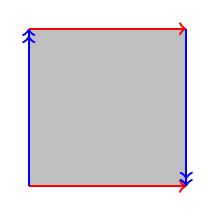
\begin{tikzpicture}
        \fill[color=black!25] (0,0) rectangle (2,2);
        \draw[thick,->, red] (0,0) -- ++(2,0);
        \draw[thick,->,red] (0,2) -- ++(2,0);
        \draw[thick,->>, blue] (0,0) -- ++(0,2);
        \draw[thick,->>,blue] (2,2) -- ++(0,-2);
    \end{tikzpicture}};

    \node (Tv) at (-3,-3) {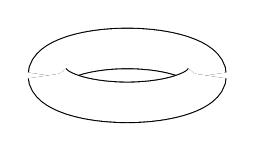
\begin{tikzpicture}[yscale=cos(70)]
        \draw[double distance=5mm] (0:1) arc (0:180:1);
        \draw[double distance=5mm] (180:1) arc (180:360:1);
      \end{tikzpicture}};
    \node (Kv) at (3,-3) {\begin{tikzpicture}[scale=0.25,use Hobby shortcut]
        \draw ([closed,blank=soft]0,0)
        \foreach \pt in {
        (-2,2),
        (2,2),
        (2,-2),
        (-2,-2),
        ([blank]-2,-1),
        (-1,-1),
        (1,-2),
        ([blank=soft]1,2),
        ([blank=soft]-1,1),
        (-3,3),
        (6,4.5),
        (4.5,-4.5),
        (-2.5,-6)
        } {
        .. ++\pt
        };
        % \draw[dashed,use previous hobby path={invert soft blanks}];
        \draw (0,0) .. +(-1,-1) .. ++(-2,-1);
        \draw[dashed] (0,0) .. +(-1,-.75) .. ++(-2,-1);
        \draw (-2.45,-3.9) .. +(3.3,-.75) .. (4.2,-3.95);
        \draw[dashed] (-2.45,-3.9) .. +(4.3,.5) .. (4.2,-3.95);
        \end{tikzpicture}};

        \draw[thick,->] (T) -- (Tv);
        \draw[thick,->] (K) -- (Kv);
    \end{tikzpicture}
    \caption{A torus and Klein bottle, with thanks to 
    \url{https://tex.stackexchange.com/q/77606/86}.}\label{fig:vanKampen}
\end{figure}

Switch to topology.   Roll up a stretchy sheet of plastic along the following 
Van Kampen diagrams  viewed in Figure~\ref{fig:vanKampen} to make a torus $\mathbb{T}^2$ 
and a Klein bottle $\mathbb{K}$.  These are different, right?  Why?  Of course we use topology 
to prove the interesting bits.  In brief, the Seifert-van Kampen theorem applies: 
the loops $\pi_1(M^2)$ on a surfaces $M^2$ can each be decomposed into an 
equivalent sequence of blue loops $b$ and red loops $r$ as shown on Figure~\ref{fig:vanKampen}.
Loops that contract to nothing can therefore be understood as running forward
along blue and red loops in some order before reversing that whole process.  In particular
the loops along the boundary do just that.  
\begin{align*}
    \pi_1(\mathbb{T}^2) &= \text{ words over }\{b,r\} \text{ rewritten by }br=rb;
    \\
    \pi_1(\mathbb{K}^2) &= \text{ words over }\{b,r\} \text{ rewritten by } r=brb. 
\end{align*}
We use algebra to compute that those groups of loops are not the same so neither are the two spaces.

Other fields?  How many times in applied math, number theory, or combinatorics
do we end up solving something even if just a linear equation, or eigenvalue?  You don't have to be convinced but the evidence is there.

Yet most of us do not want to be computers.  So what does an algebraist do 
when the questions come down to computing?  We put our energy into crafting 
algorithms to solve these problems.  In fact the word ``algorithm'' comes 
from al Khwarizmi whose influential book \emph{al Jabr} (the method of parts)
gave us the first detailed explanations of algebra.  Half of that book 
is a list of story problems solved by various algorithms in algebra.
\begin{quote}
    \textbf{The second method of algebra is to produce algorithms 
    that return solutions efficiently.}
\end{quote}

% If you are concerned that this now trends to computer science, well know that 
% computer science cares more about the data structures than about any algorithms.
% Just like counting get faster with an abacus, algebraic algorithms get better 
% with data structures.  So these two worlds interact but care deeply about 
% different parts of the problem.

\section{Relating solutions}
Sometimes we cannot find a number system to solve an equation
in a meaningful way.  Sometimes we know solutions exist but are stymied 
when it comes to finding efficient algorithms to get them.  For centuries 
no one knew if we could trisect an angle by ruler and compass and no one 
could find a general formula for factoring 4th degree polynomials.  And other 
times we succeed far too well creating far too many solutions, 
maybe infinitely many, and we simply cannot expend the time to use them all.
This is when algebra turns its interest to relating solutions to one another.

The simplest example is solving systems of linear equations.  Often 
this is in an infinite solution set.  We dampen that by describing all 
solution with a basis, and prove that any two bases are interchangeable.
A harder example are the roots of a polynomial.  Surely we have come 
to expect that roots of quadratics like $x^2-2$ will be related, 
as $x=\pm \sqrt{2}$, and more generally $x^2+x+1$ gives 
$x=z,\bar{z}$ where $z=\frac{1}{2}+\frac{\sqrt{3}i}{2}$.  That process 
generalizes and gives away an inductive process to factor many polynomials.
Lagrange used that to finally  find a general formula for quartic polynomials.
Gauss used that idea to prove that the constructable numbers (numbers we can 
produce by ruler and compass) are limited to iterations with square roots.
That explain why so many regular polygons need more than a ruler and compass 
to be drawn.  Of course we can trisect angles with 
other tools it just means ruler and compass is not enough.

The mindset of investigating relationships between solutions even leads to
identifying obstacles to having solutions.  Abel found $x^5-x-1$ could not be
solved by radicals alone.  That is, a calculator that can correctly solve
quintic or higher degree polynomials will need buttons beyond the square-root,
cube-root and n-th root buttons.  Galois went further and described exactly what
polynomials need new methods to make roots.  In a sense, Abel and Galois
explained we need to go back and invent more numbers.

\begin{quote}
    \textbf{The thrid method of algebra is to relate solutions to one another.}
\end{quote}


\section{The big picture}
Basic though it may seem, the combined model of algebra is to sequence the 
invention of new numbers, learn to compute with them, find relatinships 
between solutions, and use that to reinvent numbers.
\begin{center}
    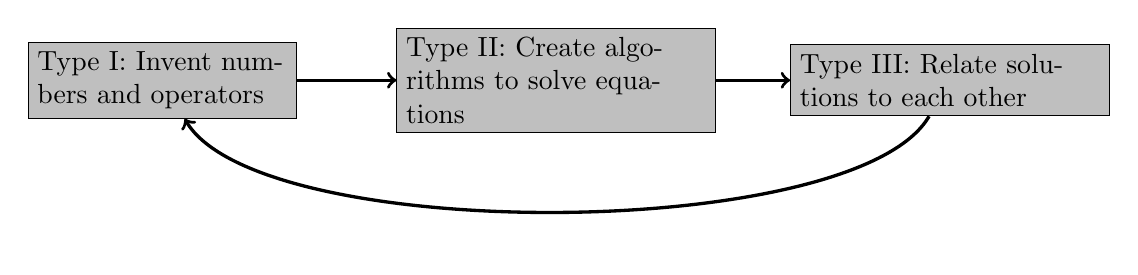
\begin{tikzpicture}
        \node[text width=1.25in, draw,fill=black!25] (a) at (0,0) {Type I: Invent numbers and operators};
        \node[text width=1.5in, draw,fill=black!25] (b) at (5,0) {Type II: Create algorithms to solve equations};
        \node[text width=1.5in, draw,fill=black!25] (c) at (10,0) {Type III: Relate solutions to each other};
        % \draw[very thick,->] (-4,0) -- (a);
        \draw[very thick,->] (a) -- (b);
        \draw[very thick,->] (b) -- (c);
        \draw[very thick,->] (c) edge[looseness=0.5,out=-120,in=-60] (a);
    \end{tikzpicture}
\end{center}


Yet to get started we better understand what it means to substitute 
for variables that can be $+$ signs and $=$ signs.